\section{Preliminaries}
\label{sec:Preliminaries}
\subsection{Problem Definition}
The traffic classification in this paper refers to classifying the encrypted traffic of sessions into specific traffic types with raw features of packets.  
Assume that there are $N$ samples and $M$ types of traffic in total.  
Let the sequence of the $p$-th sample be $\mathbf{x^{(p)}} = [\mathbf{L_1^{(p)}}, \mathbf{L_2^{(p)}}, ..., \mathbf{L_T^{(p)}}]$, where $T$ is the time sequence length of each sample and $\mathbf{L_i^{(p)}} \in \mathbb{R}^d$ is the packet feature at time step $i$.  
The traffic type of $\mathbf{x^{(p)}}$ is denoted as $y^{(p)}$, $0 \le y^{(p)} < M$. 
We consider an incremental learning scenario and aim to build an end-to-end incremental model $\psi{(\mathbf{x^{(p)}})}$ to predict a label $\hat{y_p}$ that is exactly the real label $y_p$. 
Suppose that there are total $S$ sequential stages in the learning process. 
We define stage $s$ as introducing the new class $C^s$ using the dataset $D^s = \{(\mathbf{x}, y) | y \in C^s\}$.
The training samples and labels are defined as $X^s = \{\mathbf{x}|(\mathbf{x}, y) \in D^s\}$ and $y^s = \{y|(\mathbf{x}, y) \in D^s\}$, respectively.
Especially, $y^i \cap y^j = \emptyset$ for $i \neq j$.
At stage 0, a classification model $\psi^0(\mathbf{x^{(p)}})$ is trained on dataset $X^0$ with $m^0$ classes. 
For stage $j$ a model $\psi^j(\mathbf{x^{(p)}})$ is trained to classify on accumulated $M=\sum_{q=0}^j |m^q|$ classes. 

\subsection{Long Short-Term Memory (LSTM)}
\begin{figure}[htbp]
	\centering
	\subfloat[Traditional LSTM For Classification]{
	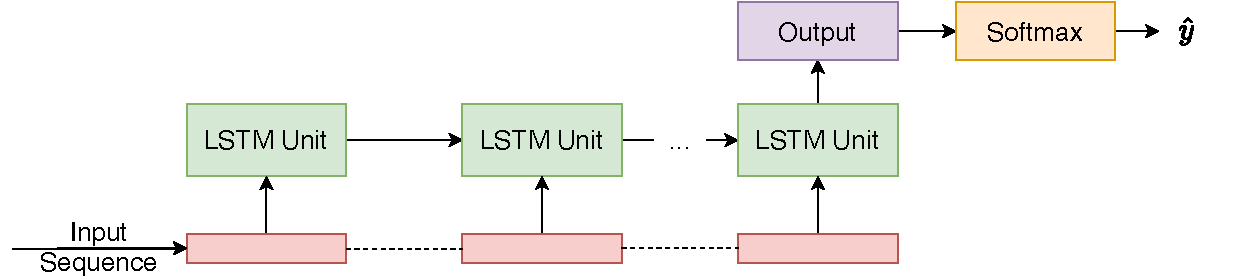
\includegraphics[scale=0.45]{figs/traditional_lstm.pdf}
	\label{fig:LSTM_a}
}\\
	\subfloat[Fingerprint LSTM For Classification]{
	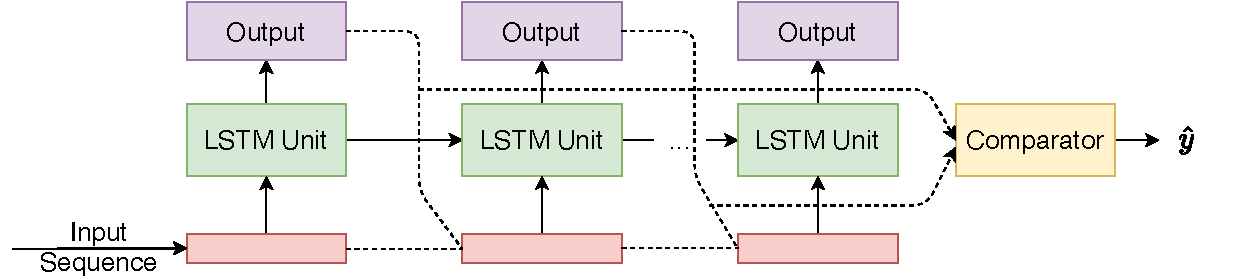
\includegraphics[scale=0.45]{figs/fingerprint_lstm.pdf}
	\label{fig:LSTM_b}
}
	\caption{Comparison between traditional LSTM and fingerprint LSTM.}
	\label{fig:LSTM}
\end{figure}
The LSTM~\cite{hochreiter1997long} is one of the most popular recurrent neural networks (RNNs)~\cite{mandic2001recurrent} to model sequential data. 
LSTM can infer the current state based on the previous state and the current input. 
Therefore, LSTM can remember past information, which is naturally suitable for sequence modeling. 
The main weak point of the vanilla version of RNN is the vanishing/exploding gradient problem which means cannot retain long-term information~\cite{bengio1994learning}. 
By adding gate units with different functions, the LSTM solves the problem. 
It can control the information transformation between the hidden states and track the states of the input sequences without using separate memory cells. 

Traditionally, as shown in Fig.~\ref{fig:LSTM_a},  when LSTM is used for classification tasks, the input sequence is first fed into the LSTM unit. 
Secondly, the output of the last time step of the LSTM unit is given to the fully connected layer.
The classification results can be get after the calculation of the softmax layer. 
However, in this paper, we use our proposed fingerprint LSTM instead of traditional LSTM. 
As shown in Fig~\ref{fig:LSTM_b}, the fingerprint LSTM tries to capture the fingerprints of different types. 
It calculates and compares the loss between the output of the current state and the input of the next time step. 
In the classification stage, the prediction results are determined by the fingerprint LSTM with the minimum loss.
There are two main benefits of fingerprint LSTM. 
First, the traditional LSTM only uses the output of the last time step for the calculation of the fully connected layer. 
Therefore, the traditional LSTM model tends to learn the features of the subsequent input. 
It can be easily affected by noise in the later-arrived packets. 
In the contrast, the learning process of the fingerprint LSTM makes the output of each time step (except the last time step) as close as possible to the input of the next time step. 
This process makes full use of all packets in a session and thus has local robustness. 
Second, a fingerprint LSTM module only characterizes the packet sequence of a specific traffic type. 
The modeling process will not be influenced by other traffic types. 
In the contrast, traditional LSTM may have a bias towards traffic types with a large number of samples.